\documentclass{report}
\usepackage{graphicx}
\usepackage{hyperref}
\usepackage{float}
\usepackage{booktabs} % For professional table formatting
\usepackage{array}    % For better column control
\usepackage{multirow} % For multi-row cells (if needed)
\usepackage{amssymb} % Pour le symbole de validation
\usepackage{pifont}  % Pour le symbole d'annulation

\title{Rapport de Projet de Fin d'Études : Développement d'un système de collecte de données en temps réel et de gestion des alertes pour les machines en salle de réveil}
\author{Zaibi Racha}
\date{\today}

\begin{document}
\setlength{\tabcolsep}{10pt} % Pour augmenter l'espacement des colonnes des tableaux
\renewcommand{\arraystretch}{1.5} % Pour augmenter l'espacement des lignes des tableaux

\maketitle

\tableofcontents
\newpage

% Introduction Générale% Import the introduction content
\section*{Introduction Générale}
\addcontentsline{toc}{section}{Introduction Générale}
Dans un contexte médical en constante évolution, l'optimisation de la surveillance des patients en salle de réveil constitue un enjeu crucial pour assurer des soins de qualité et réactifs. Actuellement, dans de nombreux établissements de santé en Tunisie, cette surveillance repose encore largement sur des méthodes manuelles et des systèmes centralisés limités, rendant difficile une détection rapide et efficace des situations critiques. Ce constat met en lumière l'importance de moderniser les processus de suivi post-opératoire à l’aide de technologies avancées et interconnectées.

Le présent projet, réalisé au sein du SmartLab de la Faculté de Médecine de Monastir, s’inscrit dans cette démarche d’innovation. Il vise à développer un système de collecte de données en temps réel et de gestion des alertes pour les machines utilisées en salle de réveil. Ce système repose sur une approche combinant l’extraction de données via la reconnaissance optique de caractères (OCR) à l’aide de caméras pour les machines ne disposant pas d’interfaces de communication.

L’objectif principal est d’assurer une prise en charge rapide et ciblée des patients en situation critique, en réduisant les délais d’intervention grâce à une détection automatisée des alertes. En intégrant des technologies web et mobiles, ce système ambitionne d’améliorer significativement la qualité des soins post-opératoires, tout en diminuant la charge de travail manuelle et le risque d’erreurs humaines.

Ainsi, ce projet répond à un besoin concret et urgent dans le domaine de la santé en proposant une solution intelligente, adaptable et évolutive, capable d’apporter une plus grande réactivité et efficacité dans la gestion des soins en salle de réveil.
 % Include the content of introduction.tex

% Cadre Général de Projet
\chapter{Cadre Général de Projet}

\section{Présentation de l’organisme d’accueil}
Le projet a été mené dans \textbf{SmartLab} de la \textbf{Faculté de médecine de Monastir (FMM)}. La Faculté de médecine de Monastir est une faculté tunisienne créée le 15 août 1980, dédiée à l’enseignement médical et à la recherche scientifique. Reconnue pour son engagement envers l’excellence, FMM a obtenu une accréditation internationale et la certification \textbf{ISO 21}, soulignant son rôle de leader dans l’éducation médicale et la recherche.

\textbf{SmartLab} est une \textbf{Unité de Service Commun et de Recherche (USCR)} de pointe associée à FMM, qui se concentre sur la promotion de l’innovation dans les sciences de la santé par le biais d’efforts de collaboration entre le secteur des soins de santé et les start-ups. En intégrant la recherche, la technologie et l’entrepreneuriat, SmartLab vise à faire progresser les soins médicaux et à créer des solutions adaptées aux défis de la santé moderne. Il sert de plaque tournante pour une collaboration interdisciplinaire, en tirant parti de l’expertise pour combler les lacunes entre la recherche et les applications réelles, contribuant ainsi à l’évolution d’une nouvelle ère en médecine.
\begin{figure}[h]
    \centering
    \begin{minipage}{0.45\textwidth}
        \centering
        
\includegraphics[width=\linewidth]{chapter1/images/logo1-fmm.png}
        \caption{Logo FMM}
    \end{minipage}
    \hfill
    \begin{minipage}{0.45\textwidth}
        \centering
        \includegraphics[width=\linewidth]{chapter1/images/logo2-smartlab.png}
        \caption{Logo SmartLab}
    \end{minipage}
\end{figure} % Use \input instead of \include

\section{Présentation de projet}

Fournissez une vue d'ensemble du projet :
\begin{itemize}
    \item \textbf{Titre} : Développement d'un système de collecte de données en temps réel et de gestion des alertes pour les machines en salle de réveil.
    \item \textbf{Objectif} : Améliorer les soins aux patients en assurant des réponses rapides aux situations critiques et en augmentant l'efficacité du personnel médical.
    \item \textbf{Portée} : Collecte de données à partir des moniteurs Mindray et des machines plus anciennes utilisant une solution basée sur caméra, gestion des alertes et notification du personnel médical.
\end{itemize} % Use \input instead of \include


\section{Étude de l’existant}

% Subsection 1.3.1: Présentation de l’étude de l’existant
\subsection{Présentation de l’étude de l’existant}
Dans les hôpitaux et cliniques en Tunisie, il n’existe actuellement \textbf{aucun système de collecte de données automatisé} en salle de réveil. Le fonctionnement repose sur :
\begin{itemize}
    \item \textbf{Un écran de surveillance centralisé} installé dans une salle administrative, permettant au personnel de suivre les signes vitaux de plusieurs patients à distance.
    \item \textbf{Une surveillance manuelle régulière} : Le personnel médical (infirmiers et médecins) doit se déplacer physiquement d’un patient à l’autre pour vérifier les constantes vitales, ce qui entraîne des \textbf{délais} dans la détection des situations critiques.
\end{itemize}

% Subsection 1.3.2: Critiques de l’existant
\subsection{Critiques de l’existant}
% \subsubsection{Absence de collecte de données en temps réel}
% \begin{itemize}
%     \item Actuellement, \textbf{aucune donnée n’est enregistrée ou stockée} automatiquement depuis les machines en salle de réveil.
%     \item La surveillance repose uniquement sur \textbf{un écran centralisé} situé dans une salle administrative.
%     \item \textbf{Les soignants doivent vérifier manuellement} l’état des patients à intervalles réguliers, ce qui peut entraîner des \textbf{retards} dans l’identification des urgences.
% \end{itemize}

\subsubsection{Manque de réactivité et d’optimisation des alertes}
\begin{itemize}
    \item Il n’existe \textbf{aucun système de gestion des alertes} priorisant les urgences en fonction de la gravité des paramètres vitaux.
    \item Les soignants \textbf{ne reçoivent pas d’alertes sur leurs appareils mobiles}, ce qui oblige à une surveillance constante de l’écran centralisé.
    \item L’absence d’un mécanisme de tri et de priorisation des alertes peut \textbf{retarder l’intervention} sur les cas critiques.
\end{itemize}

\subsubsection{Charge de travail accrue et inefficacité opérationnelle}
\begin{itemize}
    \item La \textbf{surveillance manuelle} et les déplacements constants du personnel entraînent une \textbf{perte de temps} et augmentent la charge de travail des soignants.
    \item \textbf{Risque d’erreurs humaines} dans la détection des anomalies, surtout en cas de forte affluence ou de fatigue du personnel.
    \item L'absence de \textbf{suivi automatisé des tendances des signes vitaux} empêche une anticipation des détériorations de l’état du patient.
\end{itemize}

% Section 1.4: Solution proposée
\section{Solution proposée}
\subsection{Collecte de données}
\begin{itemize}
    \item Solution basée sur caméra pour les moniteurs des signes vitaux, combinant \textbf{OpenCV} et \textbf{Tesseract OCR} pour extraire les données des écrans.
\end{itemize}

\subsection{Gestion des alertes basée sur des règles}
\begin{itemize}
    \item Envoi des notifications via e-mails et notifications mobiles grâce au \textbf{Firebase Cloud Messaging (FCM)}.
\end{itemize}


% Section 1.5: Objectifs
\section{Objectifs}
\begin{itemize}
    \item Collecte de données en temps réel dans les salles de réveil.
    \item Livraison des alertes en fonction de seuils définis.
    \item Amélioration des temps de réponse pour les situations critiques.
    \item Automatisation et réduction des interventions manuelles dans le traitement des données et alertes.
\end{itemize}

\section{Méthodologie adoptée}
\subsection{Choix de la méthodologie}

\subsubsection{Comparaison des méthodologies courantes}

Le tableau suivant (Tableau :~\ref{tab:comparaison_methodologies}) compare les méthodologies les plus couramment utilisées dans le développement logiciel, en mettant en évidence leurs caractéristiques clés :

\begin{table}[H]
    \centering
    \begin{tabular}{|m{3cm}|c|c|c|c|}
        \hline
        \textbf{Caractéristiques} & \textbf{Scrum} & \textbf{Waterfall} & \textbf{Lean} & \textbf{Kanban} \\
        \hline
        \textbf{Adaptabilité aux changements} & \checkmark & X & X & \checkmark \\
        \hline
        \textbf{Livraisons fréquentes} & \checkmark & X & X & X \\
        \hline
        \textbf{Collaboration renforcée} & \checkmark & X & X & \checkmark \\
        \hline
        \textbf{Réponse rapide aux changements} & \checkmark & X & X & X \\
        \hline
        \textbf{Gestion des risques} & \checkmark & \checkmark & \checkmark & \checkmark \\
        \hline
        \textbf{Niveau d'implication du client} & Élevé & Faible & Moyen & Moyen \\
        \hline
        \textbf{Efficacité des coûts} & Élevée & Moyenne & Élevée & Moyenne \\
        \hline
        \textbf{Assurance qualité} & Continue & Finale & Continue & Continue \\
        \hline
        \textbf{Scalabilité} & Moyenne & Élevée & Élevée & Moyenne \\
        \hline
        \textbf{Maintenance et support} & Facile & Difficile & Facile & Facile \\
        \hline
    \end{tabular}
    \caption{Comparaison des méthodologies de développement logiciel}
    \label{tab:comparaison_methodologies}
\end{table}
\subsubsection{Conclusion}

% Comme le montre le tableau, Scrum se distingue par sa flexibilité, son approche itérative et sa capacité à s'adapter aux exigences changeantes. Ces caractéristiques sont essentielles pour le développement d'un système complexe comme celui de la collecte de données et de la gestion des alertes en salle de réveil. 
Par conséquent, Scrum est la méthodologie la plus adaptée pour ce projet.
Les principales raisons du choix de Scrum sont les suivantes :
\begin{itemize}
    \item \textbf{Adaptabilité aux changements} : Les besoins des utilisateurs et les exigences techniques peuvent évoluer au fil du projet, et Scrum permet d’y répondre efficacement.
    \item \textbf{Développement itératif} : Chaque sprint permet d’obtenir un incrément fonctionnel du produit, facilitant ainsi les tests et l’amélioration continue.
    \item \textbf{Collaboration et transparence} : Les réunions régulières favorisent la communication entre les équipes et les parties prenantes, assurant une meilleure gestion du projet.
    \item \textbf{Amélioration continue} : L’analyse régulière des performances et des difficultés permet une optimisation constante du processus de développement.
\end{itemize}

\subsection{Présentation de SCRUM}
Comme présente la figure ~\ref{fig:scrum_process}, Scrum est un framework agile qui repose sur des cycles de développement appelés \textbf{sprints}. Chaque sprint a une durée définie (généralement entre 2 et 4 semaines) et aboutit à un produit fonctionnel et potentiellement livrable.
Le processus Scrum comprend plusieurs éléments clés :
\begin{itemize}
    \item \textbf{Product Backlog} : Liste des fonctionnalités à développer, priorisée par le Product Owner en fonction des besoins des utilisateurs et des objectifs du projet.
    \item \textbf{Sprint Backlog} : Ensemble des tâches à réaliser pendant un sprint, défini par l'équipe de développement.
    \item \textbf{Sprint Planning} : Réunion permettant de définir les objectifs et les tâches du sprint.
    \item \textbf{Daily Scrum} : Brève réunion quotidienne de l'équipe pour suivre l'avancement et identifier les obstacles.
    \item \textbf{Sprint Review} : Présentation de l'incrément produit aux parties prenantes à la fin de chaque sprint.
    \item \textbf{Sprint Retrospective} : Analyse du sprint pour identifier les axes d'amélioration.
\end{itemize}

\begin{figure}[H] % Use [H] to force the figure to appear exactly here
    \centering
    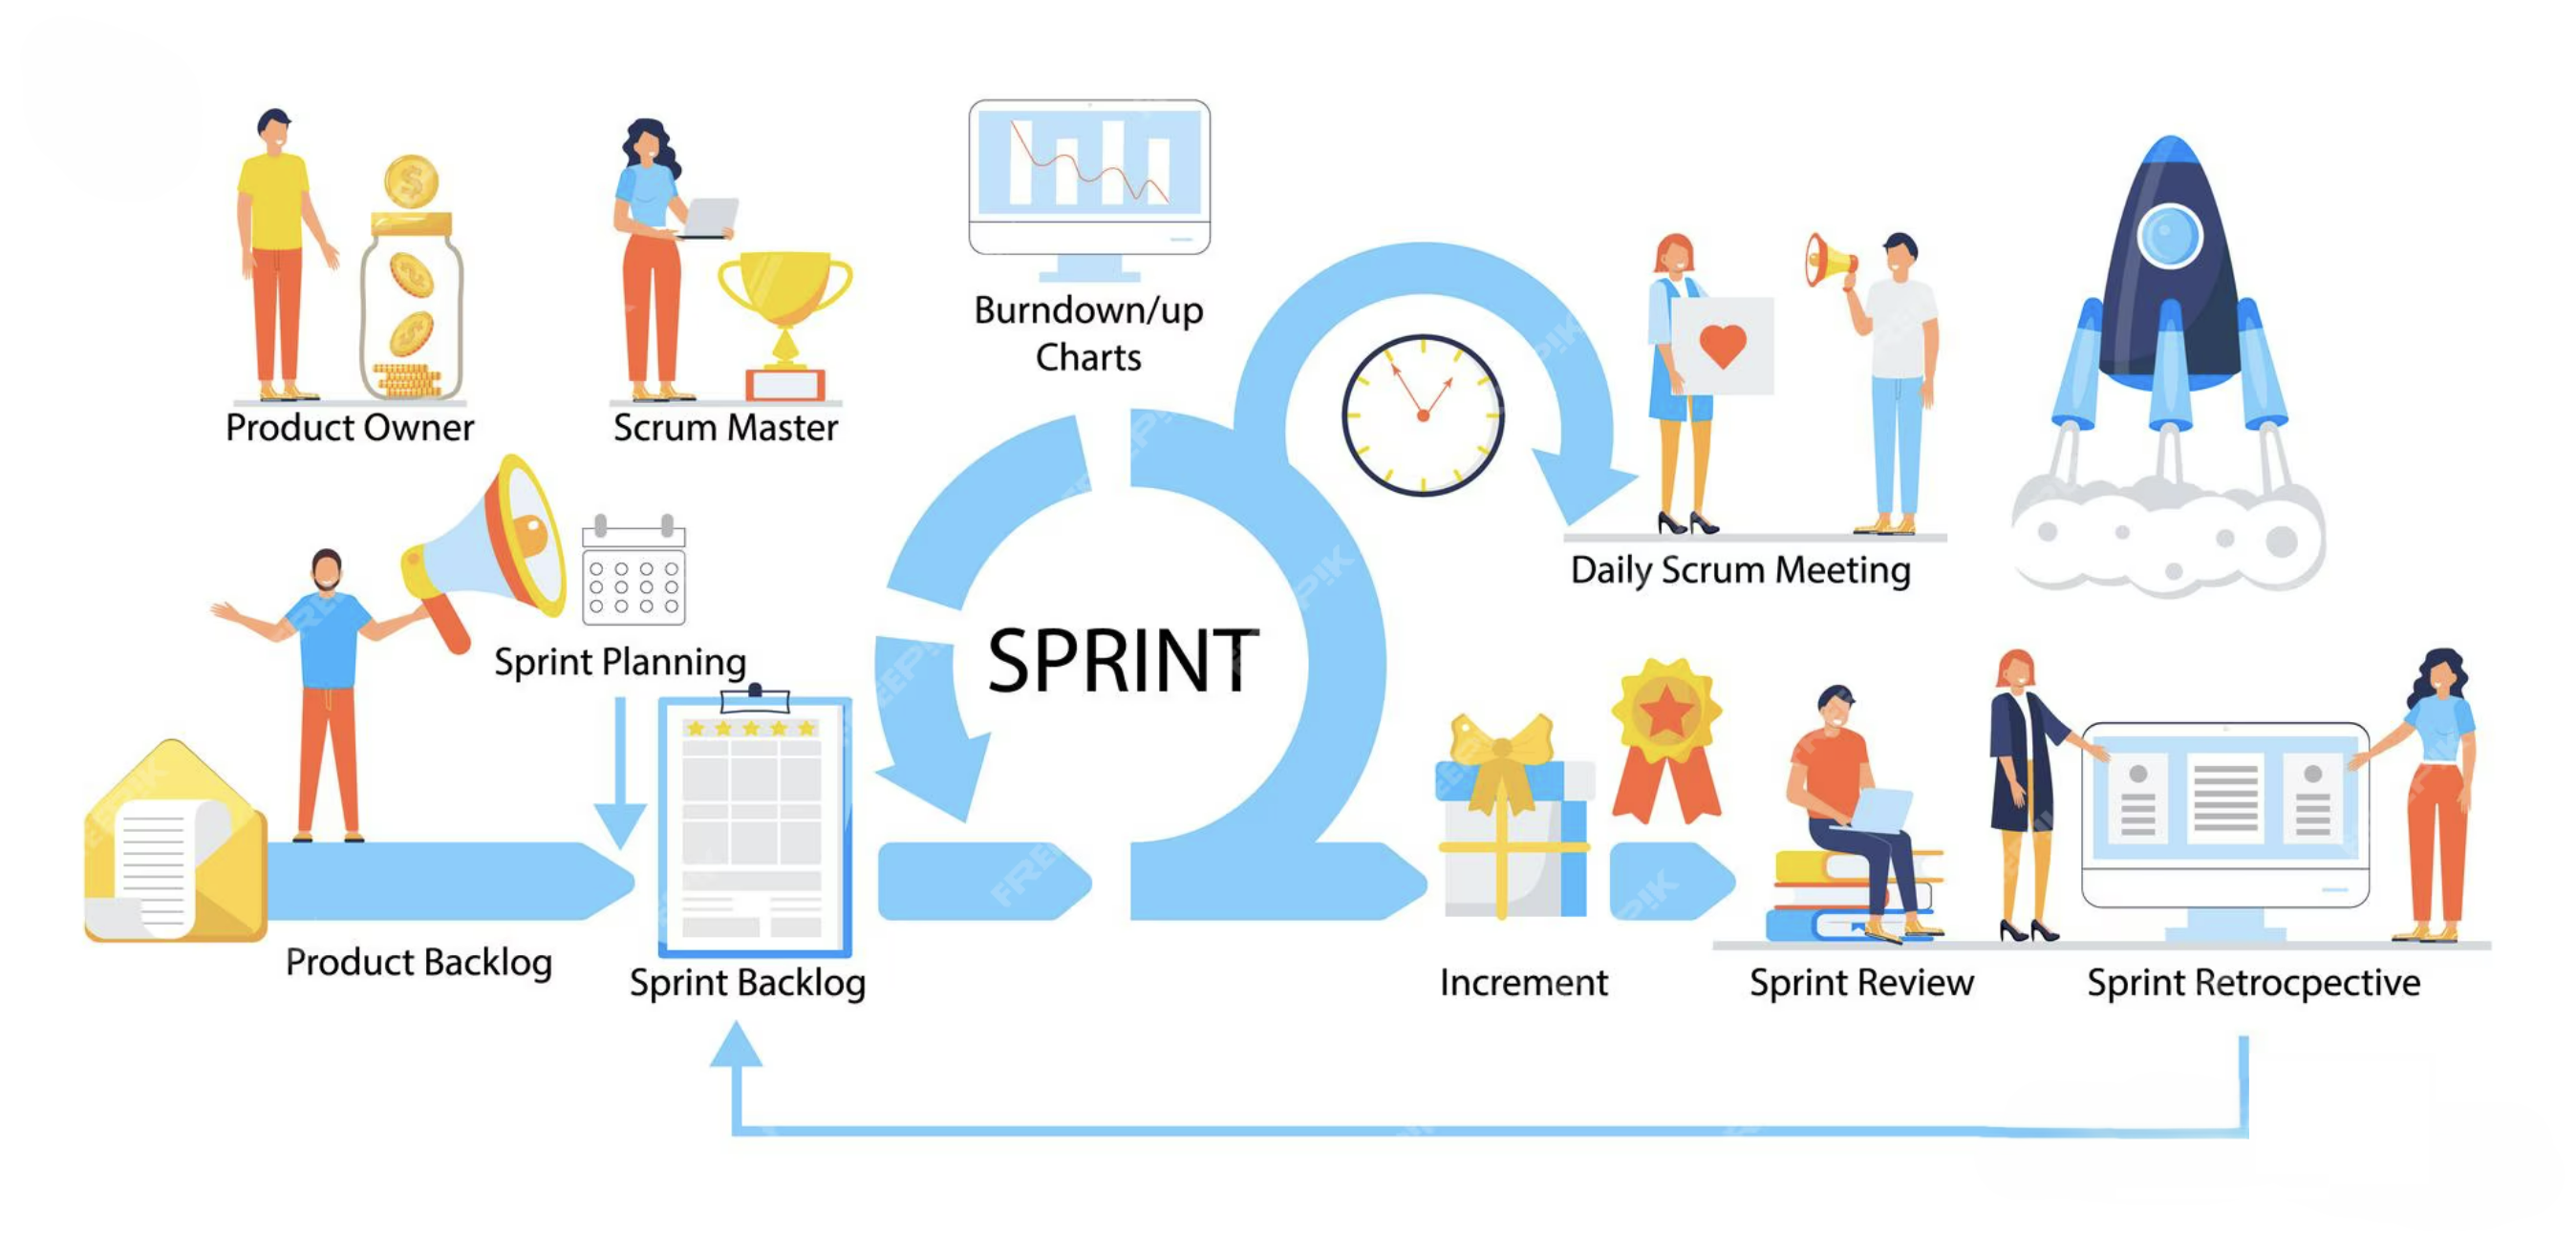
\includegraphics[width=1\linewidth]{chapter1/images/scrum.png} % Adjust width as needed
    \caption{Processus Scrum}
    \label{fig:scrum_process}
\end{figure}

\subsection{Les rôles SCRUM}
Dans Scrum, trois rôles principaux sont définis :

\begin{itemize}
    \item \textbf{Product Owner} : Représentant des parties prenantes, il définit et priorise les fonctionnalités à développer en fonction des besoins des utilisateurs et des objectifs du projet.
    \item \textbf{Scrum Master} : Responsable de la bonne application du framework Scrum. Il facilite la communication, aide à surmonter les obstacles et veille à l'amélioration continue des processus.
    \item \textbf{Équipe de développement} : Composée de développeurs, designers et autres spécialistes, elle est responsable de la mise en œuvre des fonctionnalités et de la livraison des incréments du produit.
\end{itemize}

En adoptant Scrum, le projet bénéficie d'une approche structurée et efficace, garantissant un suivi rigoureux et une réponse rapide aux exigences changeantes du domaine médical.

\begin{figure}[H] % Use [H] to force the figure to appear exactly here
    \centering
    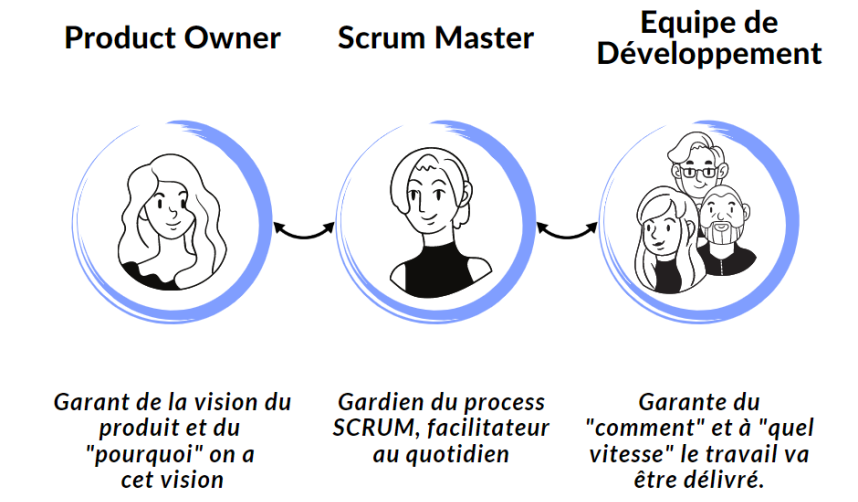
\includegraphics[width=1\linewidth]{chapter1/images/scrum-roles.png} % Adjust width as needed
    \caption{Rôles Scrum}
    \label{fig:scrum_roles}
\end{figure}


% Sprint 0
\chapter{Sprint 0}

\section{Capture des besoins}
\subsection{Identification des acteurs}
Identifiez les principales parties prenantes :
\begin{itemize}
    \item Personnel médical (médecins, infirmières).
    \item Patients.
    \item Département IT de l'hôpital.
\end{itemize}

\subsection{Identification des besoins}
Listez les exigences :
\begin{itemize}
    \item Collecte de données en temps réel.
    \item Priorisation et livraison des alertes.
    \item Intégration avec les systèmes existants de l'hôpital.
\end{itemize}

\section{Pilotage du projet avec Scrum}
\subsection{Les fonctionnalités du backlog}
Définissez les fonctionnalités pour le Product Backlog :
\begin{itemize}
    \item Collecte de données à partir des moniteurs Mindray.
    \item Collecte de données basée sur caméra pour les machines plus anciennes.
    \item Système de gestion des alertes.
    \item Livraison des notifications (e-mail, notifications dans l'application).
\end{itemize}

\subsection{Diagramme des cas d’utilisation global}
Incluez un diagramme des cas d'utilisation montrant les interactions entre les acteurs et le système.

\subsection{Planification des sprints}
Décrivez le plan des sprints :
\begin{itemize}
    \item \textbf{Sprint 1} : Collecte de données à partir des moniteurs Mindray.
    \item \textbf{Sprint 2} : Collecte de données basée sur caméra.
    \item \textbf{Sprint 3} : Système de gestion des alertes et de notification.
\end{itemize}

\subsection{Prototypage des interfaces}
Montrez les prototypes initiaux pour les interfaces du système (par exemple, visualisation des données, gestion des alertes).

\section{Environnement de travail}
\subsection{Environnement matériel}
Listez les exigences matérielles :
\begin{itemize}
    \item Moniteurs Mindray.
    \item Caméras pour les machines plus anciennes.
    \item Serveurs pour le stockage et le traitement des données.
\end{itemize}

\subsection{Environnement de développement}
Décrivez les outils de développement :
\begin{itemize}
    \item Langages de programmation : Python, Laravel, React, Flutter.
    \item Bibliothèques : OpenCV, Tesseract OCR.
\end{itemize}

\subsection{Environnement logiciel}
Listez les exigences logicielles :
\begin{itemize}
    \item Systèmes d'exploitation.
    \item Systèmes de base de données.
    \item Protocoles de communication (HL7, API).
\end{itemize}

\section{Architecture générale de l’application}
\subsection{Architecture physique}
Décrivez l'architecture physique du système :
\begin{itemize}
    \item Connexions réseau (réseau de surveillance interne, réseau de l'hôpital).
    \item Flux de données entre les appareils et le système central.
\end{itemize}

\subsection{Fonctionnement de l’architecture}
Expliquez comment l'architecture fonctionne :
\begin{itemize}
    \item Collecte de données à partir des appareils.
    \item Traitement et stockage des données.
    \item Génération et livraison des alertes.
\end{itemize}

\subsection{Spécification logicielle du système}
Fournissez les spécifications techniques pour les composants logiciels.

\section{Diagramme de déploiement}
Incluez un diagramme de déploiement montrant comment le système sera déployé dans l'environnement hospitalier.

% Sprint 1
\chapter{Étude et réalisation du Sprint 1}

\section{Backlog du sprint}
Définissez les tâches pour le Sprint 1 :
\begin{itemize}
    \item Collecte de données à partir des moniteurs Mindray.
    \item Intégration avec HL7 ou API.
\end{itemize}

\section{Spécification fonctionnelle}
\subsection{Diagramme de cas d’utilisation}
Fournissez un diagramme des cas d'utilisation pour le Sprint 1.

\subsection{Description textuelle des cas d’utilisations}
Décrivez les cas d'utilisation en détail.

\section{Conception}
\subsection{Diagrammes des séquences détaillés}
Incluez des diagrammes de séquence pour le processus de collecte de données.

\subsection{Diagramme de Classes}
Fournissez un diagramme de classes pour les composants du système.

\section{Réalisation}
\subsection{Interface d’authentification}
Montrez l'interface d'authentification.

\subsection{Interface de Création d’un modèle de cycle de vie d’un colis}
(Adaptez cette section à votre projet si nécessaire.)

\section{Test}
Décrivez le processus de test pour le Sprint 1.

% Sprint 2
\chapter{Étude et réalisation du Sprint 2}

\section{Backlog du sprint}
Définissez les tâches pour le Sprint 2 :
\begin{itemize}
    \item Collecte de données basée sur caméra.
    \item Intégration avec OpenCV et Tesseract OCR.
\end{itemize}

\section{Spécification fonctionnelle}
\subsection{Diagramme de cas d’utilisation}
Fournissez un diagramme des cas d'utilisation pour le Sprint 2.

\subsection{Description textuelle des cas d’utilisations}
Décrivez les cas d'utilisation en détail.

\section{Conception}
\subsection{Diagrammes des séquences détaillés}
Incluez des diagrammes de séquence pour le processus de collecte de données basée sur caméra.

\subsection{Diagramme de Classes}
Fournissez un diagramme de classes pour les composants du système.

\section{Réalisation}
\subsection{Interface d’affichage de la liste des colis}
(Adaptez cette section à votre projet si nécessaire.)

\subsection{Interface de recherche d’un colis}
(Adaptez cette section à votre projet si nécessaire.)

\section{Test}
Décrivez le processus de test pour le Sprint 2.

% Sprint 3
\chapter{Étude et réalisation du Sprint 3}

\section{Backlog du sprint}
Définissez les tâches pour le Sprint 3 :
\begin{itemize}
    \item Système de gestion des alertes.
    \item Livraison des notifications (e-mail, notifications dans l'application).
\end{itemize}

\section{Spécification fonctionnelle}
\subsection{Diagramme de cas d’utilisation}
Fournissez un diagramme des cas d'utilisation pour le Sprint 3.

\subsection{Description textuelle de cas d’utilisation}
Décrivez les cas d'utilisation en détail.

\section{Conception}
\subsection{Diagrammes des séquences détaillés}
Incluez des diagrammes de séquence pour le processus de gestion des alertes.

\subsection{Diagramme de Classes}
Fournissez un diagramme de classes pour les composants du système.

\section{Réalisation}
\subsection{Interface de Consultation des détails de colis avec son état courant}
(Adaptez cette section à votre projet si nécessaire.)

\subsection{Interface de Consultation les événements et les états}
(Adaptez cette section à votre projet si nécessaire.)

\subsection{Interface d’ajout une action}
(Adaptez cette section à votre projet si nécessaire.)

\subsection{Interface d’envoi un mail au client}
Montrez l'interface pour l'envoi de notifications par e-mail.

\section{Test}
Décrivez le processus de test pour le Sprint 3.

% Conclusion Générale
\chapter*{Conclusion Générale}
\addcontentsline{toc}{chapter}{Conclusion Générale}
Résumez les résultats du projet. Soulignez les avantages du système pour les soins aux patients et l'efficacité du personnel médical.

% Bibliographie
\chapter*{Bibliographie}
\addcontentsline{toc}{chapter}{Bibliographie}
Listez toutes les références utilisées dans le rapport (par exemple, documentation HL7, documentation OpenCV, manuels Mindray).

\end{document}